% !TEX TS-program = xelatex
% !BIB program = bibtex
% !TeX spellcheck = ru_RU

% About magic macros see also
% https://tex.stackexchange.com/questions/78101/

% По умолчанию используется шрифт 14 размера.
% Если Вы не влезаете в лимит страниц и нужен 12-й шрифт,
% то уберите опцию [14pt]
\documentclass[14pt, russian]{matmex-diploma-custom}

% !TeX spellcheck = ru_RU
% !TEX root = vkr.tex
% Опциональные добавления используемых пакетов. Вполне может быть, что они вам не понадобятся, но в шаблоне приведены примеры их использования.
\usepackage{tikz} % Мощный пакет для создание рисунков, однако может очень сильно замедлять компиляцию
\usetikzlibrary{decorations.pathreplacing,calc,shapes,positioning,tikzmark}

% Библиотека для TikZ, которая генерирует отдельные файлы для каждого рисунка
% Позволяет ускорить компиляцию, однако имеет свои ограничения
% Например, ломает пример выделения кода в листинге из шаблона
% \usetikzlibrary{external}
% \tikzexternalize[prefix=figures/]

\newcounter{tmkcount}

\tikzset{
    use tikzmark/.style={
            remember picture,
            overlay,
            execute at end picture={
                    \stepcounter{tmkcount}
                },
        },
    tikzmark suffix={-\thetmkcount}
}

\usepackage{booktabs} % Пакет для верстки "более книжных" таблиц, вполне годится для оформления результатов
% В шаблоне есть команда \multirowcell, которой нужен этот пакет.
\usepackage{multirow}
\usepackage{siunitx} % для таблиц с единицами измерений

% Для названий стоит использовать \textsc{}
\newcommand{\OCaml}{\textsc{OCaml}}
\newcommand{\miniKanren}{\textsc{miniKanren}}
\newcommand{\BibTeX}{\textsc{BibTeX}}
\newcommand{\vsharp}{\textsc{V$\sharp$}}
\newcommand{\fsharp}{\textsc{F$\sharp$}}
\newcommand{\csharp}{\textsc{C\#}}
\newcommand{\GitHub}{\textsc{GitHub}}
\newcommand{\SMT}{\textsc{SMT}}

\definecolor{eclipseGreen}{RGB}{63,127,95}
% \lstdefinelanguage{ocaml}{
% keywords={@type, function, fun, let, in, match, with, when, class, type,
% nonrec, object, method, of, rec, repeat, until, while, not, do, done, as, val, inherit, and,
% new, module, sig, deriving, datatype, struct, if, then, else, open, private, virtual, include, success, failure,
% lazy, assert, true, false, end},
% sensitive=true,
% commentstyle=\small\itshape\ttfamily,
% keywordstyle=\ttfamily\bfseries, %\underbar,
% identifierstyle=\ttfamily,
% basewidth={0.5em,0.5em},
% columns=fixed,
% fontadjust=true,
% literate={->}{{$\to$}}3 {===}{{$\equiv$}}1 {=/=}{{$\not\equiv$}}1 {|>}{{$\triangleright$}}3 {\\/}{{$\vee$}}2 {/\\}{{$\wedge$}}2 {>=}{{$\ge$}}1 {<=}{{$\le$}} 1,
% morecomment=[s]{(*}{*)}
% }

\makeatletter
\@ifclassloaded{beamer}{
    %%% Обязательные пакеты
    %% Beamer
    \usepackage{beamerthemesplit}
    \usetheme{SPbGU}
    \beamertemplatenavigationsymbolsempty
    \usepackage{appendixnumberbeamer}

    %% Локализация
    \usepackage{fontspec}
    \setmainfont{CMU Serif}
    \setsansfont{CMU Sans Serif}
    \setmonofont{CMU Typewriter Text}
    %\setmonofont{Fira Code}[Contextuals=Alternate,Scale=0.9]
    %\setmonofont{Inconsolata}
    \usepackage{polyglossia}
    \setmainlanguage{russian}
    \setotherlanguage{english}

    %% Графика
    \usepackage{pdfpages} % Позволяет вставлять многостраничные pdf документы в текст

    % Математические окружения с русским названием
    \newtheorem{rutheorem}{Теорема}
    \newtheorem{ruproof}{Доказательство}
    \newtheorem{rudefinition}{Определение}
    \newtheorem{rulemma}{Лемма}
    \usepackage{fancyvrb}
}
{}
\makeatother

\usepackage[autostyle]{csquotes} % Правильные кавычки в зависимости от языка
\usepackage{totcount}
\usepackage{setspace}
\usepackage{amsmath, amsfonts, amssymb, amsthm, mathtools} % "Адекватная" работа с математикой в LaTeX



\begin{document}
% TODO: Formatting
% !TeX spellcheck = ru_RU
% !TEX root = vkr.tex

%% Если что-то забыли, при компиляции будут ошибки Undefined control sequence \my@title@<что забыли>@ru
%% Если англоязычная титульная страница не нужна, то ее можно просто удалить.
\filltitle{ru}{
    %% Актуально только для курсовых/практик. ВКР защищаются не на кафедре а в ГЭК по направлению,
    %%   и к моменту защиты вы будете уже не в группе.
    chair              = {Программная инженерия},
    group              = {24.М71-мм},
    %
    %% Макрос filltitle ненавидит пустые строки, поэтому обязателен хотя бы символ комментария на строке
    %% Актуально всем.
    title              = {Оптимизация и распределённое выполнение сетевой симуляции в Miminet с использованием Docker},
    %
    %% Здесь указывается тип работы. Возможные значения:
    %%   production - производственная практика;
    %%   coursework - отчёт по курсовой работе (ОБРАТИТЕ ВНИМАНИЕ, у техпрога и ПИ нет курсовых, только практики);
    %%   practice - отчёт по учебной практике;
    %%   prediploma - отчёт по преддипломной практике;
    %%   master - ВКР магистра;
    %%   bachelor - ВКР бакалавра.
    type               = {practice},
    %
    %% Здесь указывается вид работы. От вида работы зависят критерии оценивания.
    %%   solution - «Решение». Обучающемуся поручили найти способ решения проблемы в области разработки программного обеспечения или теоретической информатики с учётом набора ограничений.
    %%   experiment - «Эксперимент». Обучающемуся поручили изучить возможности, достоинства и недостатки новой технологии, платформы, языка и т. д. на примере какой-то задачи.
    %%   production - «Производственное задание». Автору поручили реализовать потенциально полезное программное обеспечение.
    %%   comparison - «Сравнение». Обучающемуся поручили сравнить несколько существующих продуктов и/или подходов.
    %%   theoretical - «Теоретическое исследование». Автору поручили доказать какое-то утверждение, исследовать свойства алгоритма и т.п., при этом не требуя написания кода.
    kind               = {solution},
    %
    author             = {Альшаеб Басель},
    %
    %% Актуально только для ВКР. Указывается код и название направления подготовки. Типичные примеры:
    %%   02.03.03 \enquote{Математическое обеспечение и администрирование информационных систем}
    %%   02.04.03 \enquote{Математическое обеспечение и администрирование информационных систем}
    %%   09.03.04 \enquote{Программная инженерия}
    %%   09.04.04 \enquote{Программная инженерия}
    %% Те, что с 03 в середине --- бакалавриат, с 04 --- магистратура.
    specialty          = {09.04.04 \enquote{Математическое обеспечение и администрирование информационных систем}},
    %
    %% Актуально только для ВКР. Указывается шифр и название образовательной программы. Типичные примеры:
    %%   СВ.5162.2020 \enquote{Технологии программирования}
    %%   СВ.5080.2020 \enquote{Программная инженерия}
    %%   ВМ.5665.2022 \enquote{Математическое обеспечение и администрирование информационных систем}
    %%   ВМ.5666.2022 \enquote{Программная инженерия}
    %% Шифр и название программы можно посмотреть в учебном плане, по которому вы учитесь.
    %% СВ.* --- бакалавриат, ВМ.* --- магистратура. В конце --- год поступления (не обязательно ваш, если вы были в академе/вылетали).
    programme          = {ВМ.5666.2024 \enquote{Технологии программирования}},
    %
    %% Актуально всем.
    %% Должно умещаться в одну строчку, допускается использование сокращений, но без переусердствования,
    %% короткая строка с большим количеством сокращений выглядит странно
    %supervisorPosition = {проф. кафeдры системного программирования, д.ф.-м.н.,}, % Терехов А. Н.
    %supervisorPosition = {ст. преподаватель кафедры ИАС, к.~ф.-м.~н. (если есть),}, % Смирнов К. К.
    supervisorPosition = {ст. преподаватель кафедры ИАС, к.~ф.-м.~н.},
    supervisor         = {И. В. Зеленчук.},
    %
    %% Актуально только для практик и курсовых. Если консультанта нет или он совпадает с научником, закомментировать или удалить вовсе.
    % consultantPosition = {должность, ООО \enquote{Место работы}, степень  (если есть),},
    % consultant         = {Консультант~К.~К.},
    %
    %% Актуально только для ВКР.
    % reviewerPosition   = {должность, ООО \enquote{Место работы}, степень (если есть),},
    % reviewer           = {Рецензент~Р.~Р.},
}

% Английский титульник нужен только для ВКР, остальные виды работ могут его смело игнорировать.
\filltitle{en}{
    chair              = {Advisor's chair},
    group              = {ХХ.BХХ-mm},
    title              = {Template for SPbU qualification works},
    type               = {bachelor},
    author             = {FirstName Surname},
    %
    %% Possible choices:
    %%   02.03.03 \foreignquote{english}{Software and Administration of Information Systems}
    %%   02.04.03 \foreignquote{english}{Software and Administration of Information Systems}
    %%   09.03.04 \foreignquote{english}{Software Engineering}
    %%   09.04.04 \foreignquote{english}{Software Engineering}
    %% Те, что с 03 в середине --- бакалавриат, с 04 --- магистратура.
    specialty          = {02.03.03 \foreignquote{english}{Software and Administration of Information Systems}},
    %
    %% Possible choices:
    %%   СВ.5162.2020 \foreignquote{english}{Programming Technologies}
    %%   СВ.5080.2020 \foreignquote{english}{Software Engineering}
    %%   ВМ.5665.2022 \foreignquote{english}{Software and Administration of Information Systems}
    %%   ВМ.5666.2022 \foreignquote{english}{Software Engineering}
    programme          = {СВ.5162.2020 \foreignquote{english}{Programming Technologies}},
    %
    %% Note that common title translations are:
    %%   кандидат наук --- C.Sc. (NOT Ph.D.)
    %%   доктор ... наук --- Sc.D.
    %%   доцент --- docent (NOT assistant/associate prof.)
    %%   профессор --- prof.
    supervisorPosition = {Sc.D, prof.},
    supervisor         = {S.S. Supervisor},
    %
    consultantPosition = {position at \foreignquote{english}{Company}, degree if present},
    consultant         = {C.C. Consultant},
    %
    reviewerPosition   = {position at \foreignquote{english}{Company}, degree if present},
    reviewer           = {R.R. Reviewer},
}

\maketitle
\setcounter{tocdepth}{2}
\tableofcontents

% !TeX spellcheck = ru_RU
% !TEX root = vkr.tex

\section*{Введение}
\thispagestyle{withCompileDate}
% 1- training in univer hard with buying equep and cisco went out
% 2- course with practical with link
% 3- people teaching this yandex metric : link
% 4- proplem inside the lecture all student test the lecture and students wait too much time



Обучение компьютерным сетям играет ключевую роль в подготовке специалистов по программной инженерии, системному администрированию и других направлений, связанных с разработкой и эксплуатацией информационных систем.
Для эффективного освоения этой области необходимо не только изучение теории, но и практическая работа с сетевыми конфигурациями.
Однако использование физического оборудования для обучения зачастую связано с высокими затратами и сложностью организации.

Для решения этой проблемы многие университеты используют эмуляторы, которые позволяют моделировать сетевые взаимодействия и проводить практические занятия без необходимости в реальном оборудовании.
Одним из таких инструментов является Miminet\cite{miminet}, разработанный на базе Mininet\cite{mininet}. Miminet\cite{miminet} позволяет создавать, конфигурировать и тестировать сети в виртуальной среде, что делает его доступным и удобным для образовательных целей.

Несмотря на явные преимущества использования эмуляторов, в Miminet\cite{miminet} существует проблема с долгим временем ожидания, которая ограничивает эффективность обучения. Когда большое количество студентов одновременно выполняет задания в эмуляторе, каждый из них должен ждать своей очереди, что существенно замедляет процесс обучения.
Эта проблема усугубляется ограничением вычислительных ресурсов, так как текущая архитектура эмулятора использует один контейнер для всех симуляций, что приводит к перегрузке системы.

В связи с этим возникает необходимость разработки решения для улучшения производительности и масштабируемости Miminet\cite{miminet}.
Для этого будет реализован механизм распределения нагрузки между несколькими контейнерами, что позволит значительно уменьшить время ожидания студентов иповысить эффективность выполнения симуляций.
В частности, система будет использовать динамическое распределение ресурсов и многопроцессорную обработку, что обеспечит более гибкое управление и оптимизацию работы эмулятора.
Эти улучшения позволят создать более стабильную и эффективную среду для обучения сетевым технологиям.

% !TeX spellcheck = ru_RU
% !TEX root = vkr2.tex

\section{Постановка задачи}
\label{sec:task}

Целью работы является оптимизация выполнения сетевых симуляций в Miminet\cite{miminet} за счёт эффективного распределения нагрузки между несколькими контейнерами Docker.
Основной задачей является увеличение масштабируемости симуляций путём равномерного распределения вычислительных ресурсов хоста без использования параллельных вычислений внутри контейнеров.

Для достижения данной цели были поставлены следующие задачи:
\begin{enumerate}
    \item Разработка архитектуры распределённого выполнения симуляций.
        \begin{itemize}
            \item Реализовать механизм запуска и управления несколькими контейнерами, выполняющими симуляции Miminet\cite{miminet}.
            \item Обеспечить взаимодействие между контейнерами и централизованный контроль выполнения задач.
        \end{itemize}
    \item Проектирование системы управления задачами и балансировки нагрузки.
        \begin{itemize}
            \item Выбрать и настроить механизм передачи задач (Celery \cite{celery} + RabbitMQ \cite{rabbitmq}).
            \item Разработать стратегию распределения симуляций между контейнерами, учитывающую доступные вычислительные ресурсы.
            \item Обеспечить возможность динамического масштабирования количества контейнеров.
        \end{itemize}
    \item Экспериментальное тестирование эффективности распределённого подхода.
        \begin{itemize}
            \item Провести сравнение с традиционным подходом выполнения симуляций в одном контейнере.
            \item Оценить влияние распределения симуляций на загрузку процессора, время выполнения и потребление памяти.
        \end{itemize}
    \item Валидация результатов и демонстрация практической применимости.
        \begin{itemize}
            \item Провести апробацию предложенного метода на тестовых сетевых топологиях различной сложности.
            \item Оценить потенциальные сценарии использования в реальных задачах сетевого моделирования.
            \item Подготовить документацию и руководство по использованию разработанной системы.
        \end{itemize}
    \item Предложенный подход позволит более эффективно использовать вычислительные ресурсы хоста, избегая перегрузки одного контейнера и обеспечивая стабильную работу симуляций при увеличении их количества.
\end{enumerate}

% !TeX spellcheck = ru_RU
% !TEX root = vkr2.tex

\section{Обзор}
\label{sec:relatedworks}

В данном разделе рассматриваются существующие решения для выполнения сетевых эмуляций, используемые технологии и их сравнительный анализ.

\subsection{Существующей архитектуры Miminet}

Miminet использует централизованную модель управления эмуляцией, где:
\begin{itemize}
    \item Вся эмуляция выполняется внутри одного контейнера Docker;
    \item Виртуальные узлы и соединения создаются с использованием Linux network namespaces и эмулируемых Ethernet-интерфейсов;
    \item Эмуляция управляется через Python\cite{python} API Mininet, обеспечивая настройку узлов, коммутаторов и маршрутизаторов;
    \item Весь процесс выполняется в одном окружении, что ограничивает масштабируемость при увеличении количества узлов;
\end{itemize}

\subsubsection{Ограничения текущей реализации}

Несмотря на преимущества контейнеризированного подхода, текущая архитектура Miminet имеет ряд ограничений, которые могут снижать эффективность работы системы.

Первое ограничение связано с \textbf{масштабируемостью}. Поскольку вся эмуляция выполняется в одном контейнере, невозможно динамически распределять нагрузку между несколькими процессами или узлами. При увеличении количества узлов нагрузка на вычислительные ресурсы хоста (CPU и RAM) возрастает, что приводит к увеличению времени выполнения эмуляции и ограничивает её масштабируемость.

- \textbf{Текущее время выполнения эмуляции}: Каждая эмуляция занимает примерно 10 секунд, с использованием 10\% CPU.

Второе ограничение касается \textbf{использования вычислительных ресурсов}. В текущей реализации все процессы эмуляции выполняются в одном потоке без задействования многопроцессорности. Это означает, что даже если хостовая машина имеет несколько доступных ядер процессора, они не используются эффективно, что снижает общую производительность.

- \textbf{Пример текущего использования ресурсов}: CPU загружен на 10\%, но при увеличении количества эмуляций и сложности сетевой топологии, эффективность использования CPU значительно снижается, что увеличивает время выполнения.

Третье ограничение относится к \textbf{сетевым аспектам}. Все контейнеры используют общий сетевой стек, что приводит к затруднениям при одновременном запуске нескольких эмуляций. Это создаёт потенциальные конфликты и снижает гибкость в управлении ресурсами сети. Кроме того, отсутствие явной сетевой изоляции делает невозможным параллельное выполнение эмуляций с разными конфигурациями.

\subsection{используемых технологий}

В данном проекте применяются следующие технологии:

\begin{itemize}
    \item \textbf{Python\cite{python}} — основной язык программирования проекта, благодаря своей читаемости, широкому сообществу и множеству библиотек.
    \item \textbf{Flask\cite{flask}} — лёгкий веб-фреймворк на Python, используемый для обработки HTTP-запросов, маршрутизации и взаимодействия с базой данных.
    \item \textbf{Jinja2\cite{jinja2}} — шаблонизатор, встроенный во Flask, позволяющий генерировать HTML-страницы на основе Python-данных.
    \item \textbf{Mininet\cite{mininet}} — инструмент для эмуляции компьютерных сетей. Используется для создания виртуальных узлов, маршрутизаторов и соединений между ними.
    \item \textbf{Docker\cite{docker}} — система контейнеризации, обеспечивающая изоляцию симуляций и упрощающее развертывание компонентов проекта.
    \item \textbf{RabbitMQ\cite{rabbitmq}} и \textbf{Celery\cite{celery}} — инструменты для управления задачами и реализации очередей. Используются для распределения симуляций между контейнерами.
    \item \textbf{SQLite\cite{sqlite}} — встроенная реляционная база данных, применяемая для хранения конфигураций и результатов симуляций.
    \item \textbf{SQLAlchemy\cite{sqlalchemy}} — ORM для Python, позволяющая удобно работать с базой данных на уровне объектов.
    \item \textbf{JavaScript\cite{javascript}}, \textbf{jQuery\cite{jquery}} и \textbf{AJAX} — используются для создания интерактивного пользовательского интерфейса и динамической загрузки данных без перезагрузки страницы.
    \item \textbf{Bootstrap\cite{bootstrap}} — CSS-фреймворк, применяемый для создания адаптивного и современного дизайна интерфейса.
\end{itemize}

\subsection{Выводы}

Текущая архитектура Miminet ограничена возможностями масштабируемости и эффективного использования ресурсов хоста.
Для устранения этих проблем необходимо перераспределить нагрузку между несколькими контейнерами, обеспечив изоляцию сетевого стека и динамическое управление эмуляциями.

% !TeX spellcheck = ru_RU
% !TEX root = vkr.tex

\section{Описание решения}
\label{sec:solution}

В рамках данной работы была реализована архитектура распределённого выполнения сетевых эмуляций в рамках проекта Miminet\cite{miminet} с использованием Docker и системы управления задачами Celery + RabbitMQ\cite{rabbitmq}.
Это позволило повысить масштабируемость платформы и сократить время ожидания запуска эмуляции для студентов.

\subsection{Разработка архитектуры распределённого выполнения эмуляций}
\label{subsec:task1}

Изначально все эмуляции в Miminet\cite{miminet} выполнялись в одном контейнере, что ограничивало масштабируемость: увеличение числа одновременных задач приводило к росту времени ожидания и перегрузке одного ядра CPU.

Предложенное решение включает запуск нескольких изолированных Docker-контейнеров, каждый из которых может выполнять одну или несколько эмуляций. Контейнеры работают независимо и получают задания из общей очереди RabbitMQ\cite{rabbitmq}, а изоляция каждой эмуляции реализована с помощью Mininet\cite{mininet}.

Каждый контейнер содержит воркер Celery\cite{celery}, получающий задачи из общей очереди. Такая схема позволяет масштабировать систему горизонтально — за счёт увеличения количества рабочих контейнеров без изменения основной логики.

\begin{figure}[H]
  \centering
  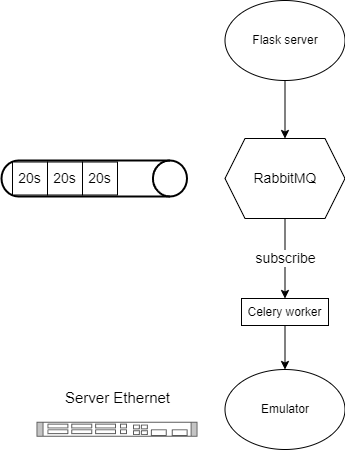
\includegraphics[width=0.40\textwidth]{figures/seq.png}
  \caption{Сравнение архитектур: исходная (один контейнер)}
  \label{fig:arch_compare}
\end{figure}

\begin{figure}[H]
  \centering
  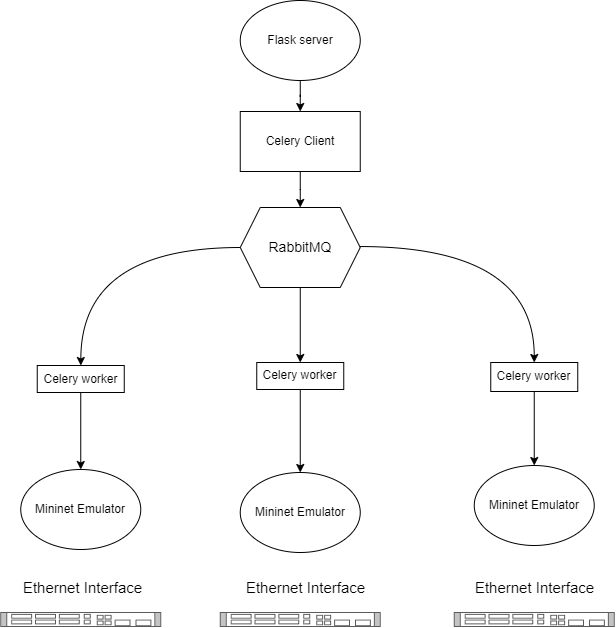
\includegraphics[width=0.60\textwidth]{figures/example.png}
  \caption{Сравнение архитектур: новая (множество контейнеров)}
  \label{fig:arch_compare}
\end{figure}

\subsection{Проектирование и внедрение системы управления задачами}
\label{subsec:task2}

Для распределения задач по контейнерам была использована связка Celery\cite{celery} + RabbitMQ\cite{miminet}.
Celery\cite{celery} позволяет организовать очередь заданий и обеспечивает параллельное выполнение с учётом текущей загрузки.

В рамках данной работы была выполнена:
\begin{itemize}
  \item настройка очереди заданий для передачи задач воркерам.
  \item параметризация контейнеров (например, через переменные окружения) для запуска с разными конфигурациями.
\end{itemize}

Каждый контейнер при старте подключается к общей очереди RabbitMQ\cite{rabbitmq} и ожидает задания.
Как только задача поступает — она исполняется и возвращает результат в центральную систему.

Такой подход позволяет эффективно масштабировать систему, добавляя или отключая контейнеры без необходимости остановки сервиса.

\subsection{Экспериментальное тестирование и валидация}
\label{subsec:task3}

Для проверки эффективности решения были проведены эксперименты с запуском 20 эмуляций в двух режимах:
\begin{itemize}
  \item один контейнер с одним воркером (исходная реализация Miminet);
  \item четыре контейнера, работающие параллельно (предложенная в рамках данной работы).
\end{itemize}

\subsubsection*{Методика}

В каждой эмуляции вручную фиксировалось время выполнения:

\begin{minted}[frame=single]{python}
import time
start = time.time()
# выполнение эмуляции
end = time.time()
print(f"Эмуляция завершена за {end - start:.2f} сек.")
\end{minted}

\subsubsection*{Метрики}
\begin{itemize}
  \item Общее время выполнения заданий.
  \item Средняя загрузка CPU.
  \item Среднее время ожидания запуска эмуляции для студентов сократилось.
  \item Количество одновременно исполняемых эмуляций.
\end{itemize}

\begin{table}[H]
\centering
\caption{Сравнение производительности}
\label{tab:cmp}
\begin{tabular}{|c|c|c|}
\hline
Конфигурация & Общее время (сек) & Ускорение \\
\hline
1 контейнер & 100 & 1.0$\times$ \\
4 контейнера & 25 & 4.0$\times$ \\
\hline
\end{tabular}
\end{table}

\begin{figure}[H]
  \centering
  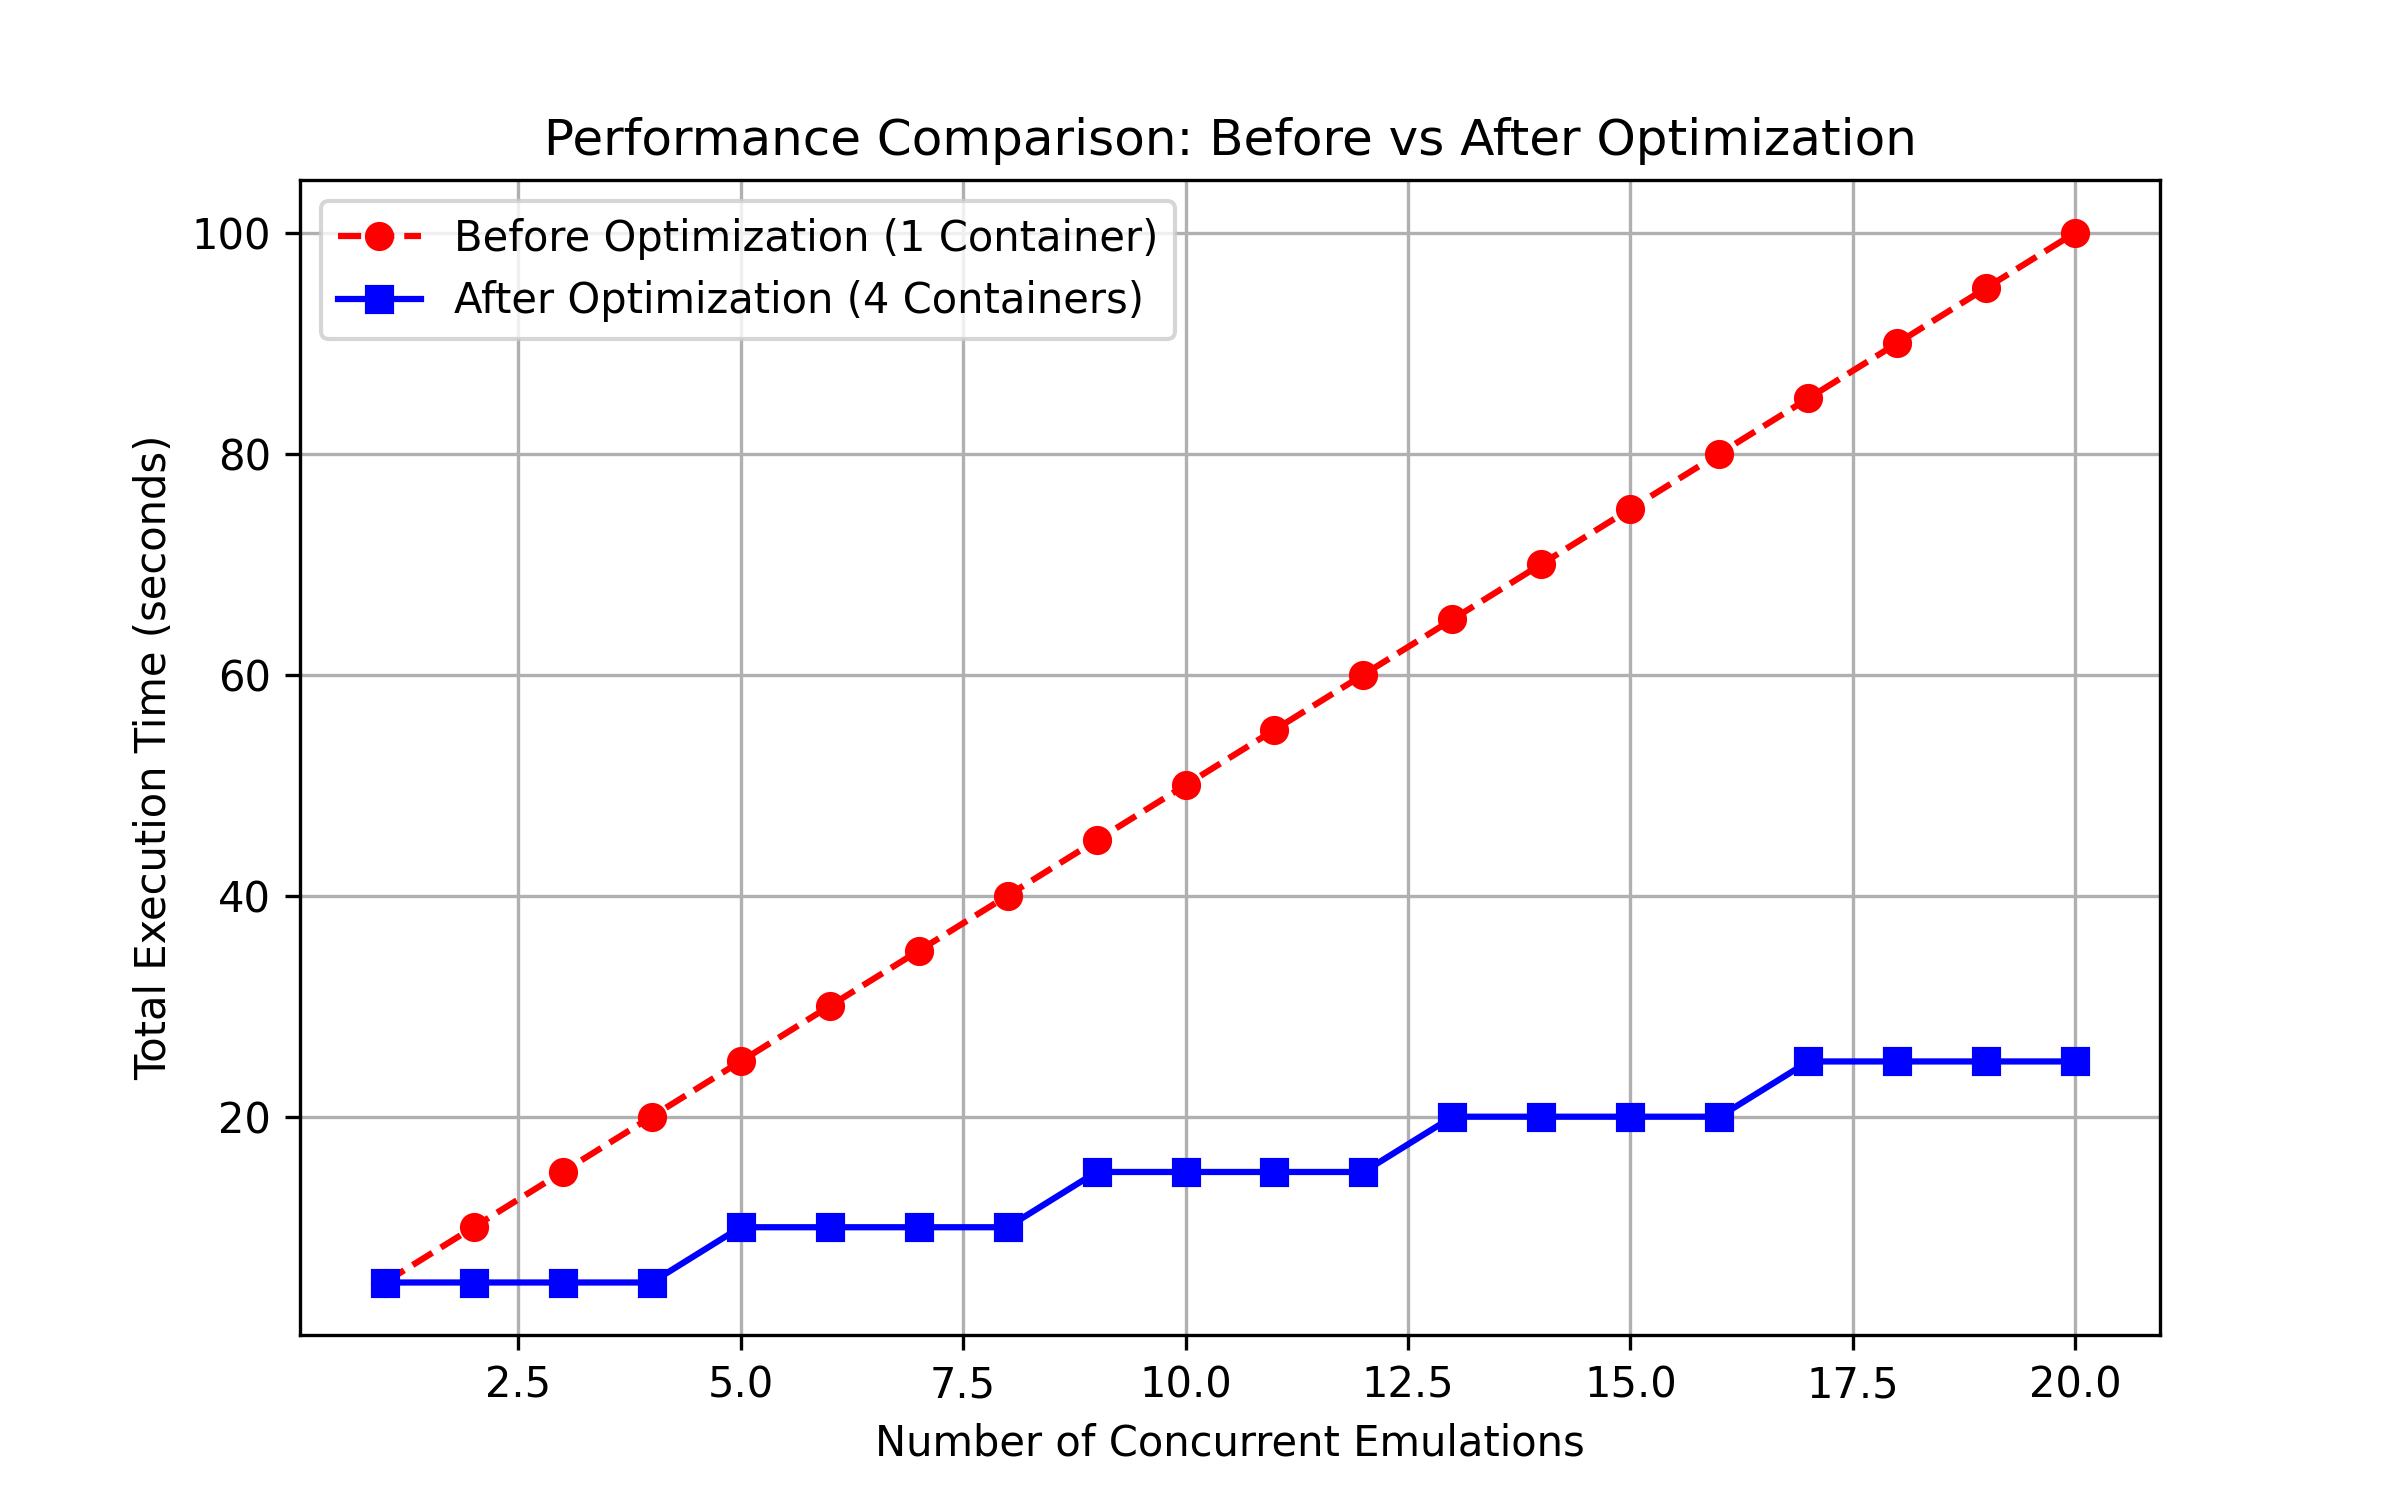
\includegraphics[width=0.75\textwidth]{figures/performance_comparison.png}
  \caption{График сравнения времени при запуске 20 эмуляций}
  \label{fig:perf}
\end{figure}

Эксперименты показали, что система с несколькими контейнерами позволяет запускать больше эмуляций одновременно и равномерно распределяет нагрузку между ядрами процессора.

Это, в свою очередь, приводит к сокращению времени ожидания и повышению эффективности обучения.

\textbf{Выводы:}
\begin{itemize}
  \item Количество параллельно исполняемых задач увеличилось в 4 раза;
  \item Загрузка CPU распределяется равномерно между ядрами;
  \item Среднее время ожидания студентом до начала эмуляции сокращается с 100 до 25 секунд.
\end{itemize}

\subsection{Итоги реализации}
\label{subsec:summary}

Предложенное решение было внедрено в существующий код проекта Miminet и протестировано в условиях, приближённых к реальному использованию студентами. Архитектура допускает дальнейшее масштабирование и автоматизацию (например, динамическое добавление контейнеров на основе текущей загрузки).

Исходный код решения доступен в открытом репозитории: \url{https://github.com/mimi-net/miminet}


\setmonofont{CMU Typewriter Text}
\bibliographystyle{ugost2008ls}
\bibliography{vkr2}

\end{document}
